\section{Greedy Algorithm with General Bids}
\label{sec:greedy_algorithm_general_bids}

In this section we revisit the Greedy algorithm of \cite{JMS02, JainMMSV03} and present its generalized version with more flexible bidding functions. The classical Greedy algorithm maintains a set $A$ of active clients, a set $S$ of opened facilities, and for each client $j$ a value $\alpha_j$ that grows uniformly while $j$ remains active. As time increases, one of two events can occur. Either some unopened facility receives enough total bids to pay for its opening cost, in which case the facility is opened, or some active client reaches an already opened facility and becomes inactive. In the standard Greedy algorithm, an active client $j$ first reserves $d(i,j)$ units of its budget to pay for connecting to a candidate facility $i$, and then contributes all of its remaining budget, namely $[\alpha_j-d(i,j)]^+$, toward opening $i$. Likewise, an inactive client that is currently connected at cost $d(j,S)$ contributes the full improvement $[d(j,S)-d(i,j)]^+$ that opening $i$ would offer.

It is therefore natural to ask what happens if clients are not forced to bid their entire remaining budget to a candidate facility, but are instead allowed to contribute only a fraction of it.
%, with this fraction depending on the distance to the candidate facility. 
Intuitively, one would like clients to support nearby facilities more aggressively and discount their bids to facilities that are farther away.

Our goal is to understand the power of the bidding function in the Greedy algorithm. For a client with value $\alpha$, we denote its bid toward a facility at distance $d$ by $\beta(\alpha,d)$, and for an inactive client we use the same function with $\alpha=d(j,S)$, namely $\beta(d(j,S),d)$. We give the pseudocode of the Generalized Greedy algorithm in Algorithm~\ref{alg:dual_generalized}. Of course, the bidding function $\beta(\alpha,d)$ must
satisfy some natural properties, e.g. the bids should be non-negative and should not surpass
the remaining budget. We outline these properties in Section~\ref{sec:natural-properties-bidding} and from this point onwards, whenever we refer to the Generalized Greedy algorithm (Algorithm~\ref{alg:dual_generalized}), we assume that its bidding function satisfies these properties.

\begin{algorithm}
\caption{Greedy Algorithm with a Generalized Bidding Strategy}
\label{alg:dual_generalized}
\begin{algorithmic}[h]
\State \textbf{Initialization:} Set $A=D$ (set of active clients), $S=\emptyset$ (set of opened facilities), $\alpha=1$ (global time).
\State For each client $j \in D$, let $\alpha_j=\alpha$ while $j \in A$, and freeze $\alpha_j$ when $j$ first becomes inactive.
\State For any client $j$ and facility $i$, define the bid:
\[
\text{bid}(j, i) = 
\begin{cases} 
\beta(\alpha_j, d(i,j)) & \text{if } j \in A \\
\beta(d(j,S), d(i,j)) & \text{if } j \notin A\,.
\end{cases}
\]
\While{$A \ne \emptyset$}
    \State Increase $\alpha$ uniformly until one of the following events occurs:
    \State \textbf{Event 1:} An unopened facility $i \in F$ is fully paid for: $\sum_{j \in D} \text{bid}(j, i) = f$
    \State \indent Open facility $i$: $S \gets S \cup \{i\}$
    \State \indent Mark all clients $j \in A$ such that $\alpha_j \geq \dist(j,S)$ as served (i.e., remove them from $A$).

    \State \textbf{Event 2:} An active client $j \in A$ reaches an open facility $i \in S$: $\alpha_j = d(i,j)$
    \State \indent Mark $j$ as served (i.e., remove $j$ from $A$).
    
    \Statex \textit{(If multiple events occur simultaneously, process them in an arbitrary order)}
\EndWhile
\end{algorithmic}
\end{algorithm}

\subsection{Motivation for General Bidding Functions}

In this section we recall the classic factor-$2$ lower bound for the standard Greedy algorithm
of \cite{JMS02, JainMMSV03} and show how a slightly different bidding function can help us break the barrier of $2$. The examples we present do not have uniform opening costs for the facilities, i.e. every facility has a different opening cost $f_i$ and it opens when
the total bids towards it are equal to $f_i$. This is done purely for presentational 
simplicity as similar examples can be obtained for uniform opening costs. Additionally,
in these examples, the quantity that ``reveals'' the LMP factor of the algorithm is the following. Let $i$ be an optimal facility with opening cost $f$, and $d_1, \dots, d_n$ 
be the distances between the facility and the clients connected to it in the optimal solution. We are interested in bounding the following ratio:
\[\frac{\sum_{j = 1}^n a_j - f}{\sum_{j = 1}^n d_j}\,.\]
\noindent The above quantity is a crucial ingredient in the analysis of the algorithm and is essentially equal to the final LMP approximation. In fact, this is exactly the objective of the Factor Revealing program developed
in \cite{JMS02, JainMMSV03} to analyze the standard Greedy algorithm.


\begin{figure}[h]
\centering
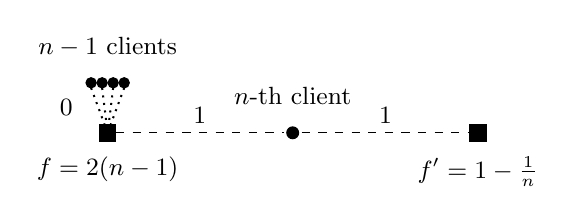
\begin{tikzpicture}[x=1cm,y=1cm,every node/.style={font=\small}]
    \def\boxsize{0.21}
    \def\dotr{0.065}
    \def\solodotr{0.075}
    \def\seglen{2.35}
    \def\basey{0.105}
    \def\clienty{0.74}
    \def\labely{0.95}
    \def\fx{0.105}
    \def\sx{\fx+\seglen}
    \def\fpx{\fx+2*\seglen}

    \filldraw[black] ({\fx-\boxsize/2},{\basey-\boxsize/2}) rectangle ({\fx+\boxsize/2},{\basey+\boxsize/2});
    \filldraw[black] ({\fpx-\boxsize/2},{\basey-\boxsize/2}) rectangle ({\fpx+\boxsize/2},{\basey+\boxsize/2});

    \filldraw[black] ({\fx-0.21},{\clienty}) circle (\dotr);
    \filldraw[black] ({\fx-0.07},{\clienty}) circle (\dotr);
    \filldraw[black] ({\fx+0.07},{\clienty}) circle (\dotr);
    \filldraw[black] ({\fx+0.21},{\clienty}) circle (\dotr);
    \node[anchor=south] at ({\fx},{\labely}) {$n-1$ clients};

    \draw[dotted, line width = 0.73pt] ({\fx-0.21},{\clienty-\dotr}) -- ({\fx},{\basey});
    \draw[dotted, line width = 0.73pt] ({\fx-0.07},{\clienty-\dotr}) -- ({\fx},{\basey});
    \draw[dotted, line width = 0.73pt] ({\fx+0.07},{\clienty-\dotr}) -- ({\fx},{\basey});
    \draw[dotted, line width = 0.73pt] ({\fx+0.21},{\clienty-\dotr}) -- ({\fx},{\basey});
    \node[anchor=east] at ({\fx-0.32},{0.5*(\clienty+\basey)}) {$0$};

    \node[anchor=north] at ({\fx},{\basey-\boxsize/2-0.08}) {$f =  2(n-1)$};

    \filldraw[black] ({\sx},{\basey}) circle (\solodotr);
    \node[anchor=south] at ({\sx},{\basey+0.24}) {$n$-th client};

    \node[anchor=north] at ({\fpx},{\basey-\boxsize/2-0.08}) {$f' = 1-\frac1n$};

    \draw[dashed] ({\fx+\boxsize/2},{\basey}) -- node[above] {$1$} ({\sx-\solodotr-0.04},{\basey});
    \draw[dashed] ({\sx+\solodotr+0.04},{\basey}) -- node[above] {$1$} ({\fpx-\boxsize/2},{\basey});
\end{tikzpicture}
\caption{A $2$ lower bound for standard Greedy with bidding function: $[\alpha-d]^+$.}
\label{fig:greedy-hard-example}
\end{figure}

In the classical tight example, depicted in  Figure~\ref{fig:greedy-hard-example}, 
we have two facilities at distance $2$ from each other with opening costs $f$ and $f'$.
The instance consists of $n-1$ clients that are co-located with the facility $f$ (i.e. at distance $0$) and one client that is at distance $1$ from both facilities.
On a high level, in this example the standard Greedy algorithm might open the facility $f'$
using only the bid of the separated client, which then forces the $n-1$ clients
to raise to a higher level in order to pay for the opening of $f$.

Indeed, when the active clients reach value $\alpha = 2-\frac1n$, the separated client bids exactly $1-\frac1n$ to both facilities, while each of the $n-1$ co-located clients bids $2-\frac1n$ to $f$ and $0$ to $f'$. Therefore, both facilities receive bids that are exactly equal to their opening costs. If Greedy chooses to open $f'$ first, then only the $n$-th client becomes inactive. The other $n-1$ clients are still at distance $2$ from the open facility, so they remain active (as their budget cannot yet pay for their connection cost) and keep increasing their values until $\alpha=2$, when they can either open facility $f$ by themselves or simply connect to $f'$.
In the resulting execution, the final client values are
\[
    \alpha_n = 2-\frac1n 
    \qquad\text{and}\qquad
    \alpha_j = 2 \quad \text{for every } j \leq n-1\,.
\]

\noindent At the same time, the optimal solution opens only $f$, paying opening cost $2(n-1)$ and connection cost $1$ for the $n$-th client. As a result, the factor of the algorithm for this example is

$$
\frac{\sum_{j = 1}^n a_j - f}{\sum_{j=1}^n d_j} = \frac{2(n-1) + 2-\frac1n - 2(n-1)}{1} = 2-\frac1n\,.
$$


Consider now a slightly different bidding rule, namely $\beta(\alpha,d)=[\alpha-(1+\eps)d]^+$, for some $\eps>0$.
The main difference is that the facility $f'$ can no longer be opened at time $\alpha = 2-\frac1n$, because the isolated client does not contribute its full remaining budget but contributes only
\[
    \left[2-\frac1n-(1+\eps)\right]^+
    =
    \left[1-\eps-\frac1n\right]^+
    <
    1-\frac1n\,.
\]
On the other hand, the facility $f$ can open as soon as $(n-1)\alpha + [\alpha-(1+\eps)]^+ = 2(n-1)$, that is, at time $\alpha = 2-\frac{1-\eps}{n}$. At this time, the facility $f'$ still does not receive enough bids, as the isolated client's contribution is
\[
    [\alpha-(1+\eps)]^+ = \frac{(n-1)(1-\eps)}{n} < 1-\frac1n\,.
\]
\noindent As a result, Greedy opens $f$ first and terminates as all the clients connect to $f$. 
Therefore, the final client values for this execution are 
\[
    \alpha_j = 2-\frac{1-\eps}{n}, \quad \text{for every } j \leq n\,.
\]
The final factor for this example is thus

$$
\frac{\sum_{j = 1}^n a_j - f}{\sum_{j = 1}^n d_j} =  n\left(2-\frac{1-\eps}{n}\right)-2(n-1)=1+\eps\,.
$$

\noindent Hence, even this simple modification already improves the first example from $2-\frac1n$ to $1+\eps$. In fact, for any $\gamma \in (1,2)$, one can follow the same analysis and get that the bidding function $[\alpha-\gamma d]^+$ yields a ratio of $\gamma$ on this example, which is strictly better than standard Greedy.


Of course, the previous example (Figure~\ref{fig:greedy-hard-example}) is tailored
to the standard Greedy algorithm, or equivalently to $\gamma = 1$, as the ``bad event'' (i.e. 
that $f'$ can be opened before $f$) only happens for $\gamma = 1$. Following the same rationale,
this example can be generalized so that $f'$ and $f$ become tight exactly at the same time for any $\gamma \in (1,2)$. We present this generalized example in Figure~\ref{fig:greedy-hard-example-gamma}.
However, even in this case the resulting ratio is $2-(1-\gamma)^2$ which is strictly better
than $2$ for any $\gamma \in (1,2)$. In fact, we later prove that the aforementioned ratio
is exactly tight for $\gamma \in (1,1.224)$; this proves that Algorithm~\ref{alg:dual_generalized} with the bidding function $\beta_{1.224}(\alpha,d) = [\alpha - 1.224 d]^+$ is a $1.95$-LMP approximation. 


\begin{figure}[h]
\centering
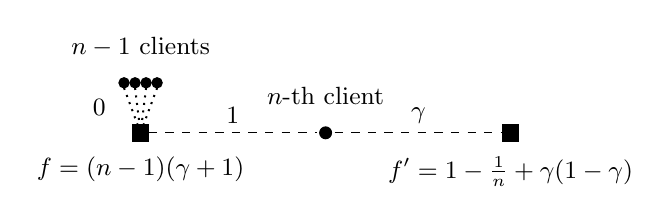
\begin{tikzpicture}[x=1cm,y=1cm,every node/.style={font=\small}]
    \def\boxsize{0.21}
    \def\dotr{0.065}
    \def\solodotr{0.075}
    \def\seglen{2.35}
    \def\basey{0.105}
    \def\clienty{0.74}
    \def\labely{0.95}
    \def\fx{0.105}
    \def\sx{\fx+\seglen}
    \def\fpx{\fx+2*\seglen}

    \filldraw[black] ({\fx-\boxsize/2},{\basey-\boxsize/2}) rectangle ({\fx+\boxsize/2},{\basey+\boxsize/2});
    \filldraw[black] ({\fpx-\boxsize/2},{\basey-\boxsize/2}) rectangle ({\fpx+\boxsize/2},{\basey+\boxsize/2});

    \filldraw[black] ({\fx-0.21},{\clienty}) circle (\dotr);
    \filldraw[black] ({\fx-0.07},{\clienty}) circle (\dotr);
    \filldraw[black] ({\fx+0.07},{\clienty}) circle (\dotr);
    \filldraw[black] ({\fx+0.21},{\clienty}) circle (\dotr);
    \node[anchor=south] at ({\fx},{\labely}) {$n-1$ clients};

    \draw[dotted, line width = 0.73pt] ({\fx-0.21},{\clienty-\dotr}) -- ({\fx},{\basey});
    \draw[dotted, line width = 0.73pt] ({\fx-0.07},{\clienty-\dotr}) -- ({\fx},{\basey});
    \draw[dotted, line width = 0.73pt] ({\fx+0.07},{\clienty-\dotr}) -- ({\fx},{\basey});
    \draw[dotted, line width = 0.73pt] ({\fx+0.21},{\clienty-\dotr}) -- ({\fx},{\basey});
    \node[anchor=east] at ({\fx-0.32},{0.5*(\clienty+\basey)}) {$0$};

    \node[anchor=north] at ({\fx},{\basey-\boxsize/2-0.08}) {$f = (n-1)(\gamma+1)$};

    \filldraw[black] ({\sx},{\basey}) circle (\solodotr);
    \node[anchor=south] at ({\sx},{\basey+0.24}) {$n$-th client};

    \node[anchor=north] at ({\fpx},{\basey-\boxsize/2-0.08}) {$f' = 1-\frac1n+\gamma(1-\gamma)$};

    \draw[dashed] ({\fx+\boxsize/2},{\basey}) -- node[above] {$1$} ({\sx-\solodotr-0.04},{\basey});
    \draw[dashed] ({\sx+\solodotr+0.04},{\basey}) -- node[above] {$\gamma$} ({\fpx-\boxsize/2},{\basey});
\end{tikzpicture}
\caption{A $2-(\gamma-1)^2$ lower bound for Greedy with the bidding rule $\beta_{\gamma}(\alpha,d)=[\alpha-\gamma d]^+$.}
\label{fig:greedy-hard-example-gamma}
\end{figure}

\vspace{1em}

We complete this section by showing that the example of Figure~\ref{fig:greedy-hard-example-gamma} gives indeed a lower bound of $2-(1-\gamma)^2-\frac1n$ for the bidding functions $\beta_\gamma(\alpha,d) = [\alpha - \gamma d]^+$ with $\gamma \in (1,2)$.


\noindent Let us define $\tau = 1+\gamma-\frac1n.$ At time $\alpha = \tau$, the co-located
clients do not yet bid towards $f'$ because $\tau - (\gamma+1) = -\frac1n < 0$.
At the same time, the isolated client bids $[\tau-\gamma^2]^+ = 1+\gamma-\gamma^2-\frac1n$ towards facility $f'$ and $[\tau-\gamma]^+ = 1-\frac1n$ towards facility $f$. Notice that at this time, both facilities can be paid for since
$$
[\tau-\gamma^2]^+ = f' \quad\text{and}\quad (n-1)\tau + [\tau-\gamma]^+ = f\,.
$$
\noindent Suppose Greedy breaks the tie by opening $f'$ first. Then the $n$-th client becomes inactive, while the other $n-1$ clients remain active because they are still at distance $1+\gamma > \tau$ from the opened facility. Moreover, the, now inactive, isolated client does not contribute to facility $f$ anymore, because its current distance to $f'$ is $\gamma$
and its bid under the bidding function is $[\gamma - 1\cdot\gamma]^+ = 0$. 
Therefore only the $n-1$ co-located clients continue to bid for $f$ and they open $f$ by time
\[
    \frac{f}{n-1} = 1+\gamma\,.
\]
At time $\alpha = 1+\gamma$, the co-located clients can either open $f$ or connect to $f'$.
Suppose that they connect to $f'$; notice that opening $f$ would result to a smaller final cost
because the isolated client would get its connection distance dropped to $1$ without extra bidding.
At the end of the execution, the $n$-th client has paid $\tau-\gamma^2$ in its first bid and
$\gamma$ for its connection cost. The $n-1$ co-located clients together pay exactly the opening cost of $f$, and therefore the factor of this example is
$$
\frac{\sum_{j = 1}^n a_j - f}{\sum_{j = 1}^n d_j} = \tau - \gamma^2 + \gamma = 2-(1-\gamma)^2 -\frac1n\,.
$$

\subsection{Properties of Bidding Functions}\label{sec:natural-properties-bidding}

We now state a number of natural structural properties that the bidding functions must satisfy. 
These are precisely the properties used later in the analysis, and they capture the basic 
intuition that bids should behave smoothly, monotonically, and consistently under rescaling.

\begin{definition}[Admissible bidding functions]
A bidding function $\beta : \reals_{\ge 0}^2 \to \reals_{\ge 0}$ must satisfy the following properties.
\begin{enumerate}
    \item \emph{Non-negative:} $\beta(\alpha,d)\ge 0$ for every $\alpha,d \ge 0$.
    \item \emph{Budget-feasible:} $\beta(\alpha,d) \leq [\alpha-d]^+$ for every $\alpha,d \ge 0$.
    \item \emph{Continuous:} $\beta$ is continuous in both arguments.
    \item \emph{Monotonic:} $\beta$ is non-decreasing in its first argument and non-increasing in its second argument.
    \item \emph{Scale equivariant:} for every $\alpha>0$ and $d\ge 0$, it holds that 
    $$ \beta(\alpha,d)=\alpha \cdot \beta(1,d/\alpha)$$
    \item \emph{Superadditive:} whenever $x_1 \ge x_2 \ge x_3 \ge 0$,
    $$
        \beta(x_1,x_2) + \beta(x_2,x_3) \le \beta(x_1,x_3).
    $$
\end{enumerate}
\end{definition}

The first four properties are immediate from the intended interpretation of a bid. A client should never make a negative contribution or contribute more than its remaining budget after paying for its distance. Bids should also not change discontinuously under an infinitesimal perturbation of either the client's value or the distance to the facility. Additionally, the monotonicity guarantees that a client with larger value should not bid less while a farther facility should also not receive a larger bid.

Scale equivariance expresses that the bidding rule should be invariant under a uniform rescaling of the metric and of the opening costs. This is natural both algorithmically and analytically: if all distances and opening costs are multiplied by the same factor, then the algorithm should simply scale its bids by the same factor and preserve the same approximation guarantee.
Finally, superadditivity formalizes the idea that reconnecting through an intermediate facility should not cost more than connecting directly to the final facility. If a client with current value $x_1$ first freezes at distance $x_2$ and later improves its connection to distance $x_3$, then the total amount it bids along this two-step process, which is $\beta(x_1, x_2) + \beta(x_2, x_3)$, should be at most the amount it would bid if it connected directly from $x_1$ to $x_3$, i.e. $\beta(x_1,x_3)$.

\paragraph{Cost of the algorithm.} Having formally defined Algorithm~\ref{alg:dual_generalized}
and the properties of the bidding function, we can now calculate the total cost in an execution of the algorithm. Fix an execution of Algorithm~\ref{alg:dual_generalized}, and let $i_0,i_1,\ldots,i_t$ be the successive facilities that strictly improve the connection of a client $j$, ordered by time of appearance. Thus
\[
    d(i_0,j) > d(i_1,j) > \cdots > d(i_t,j)\,,
\]
where $i_0$ is the facility to which $j$ first connects, and $i_t$ is the facility serving $j$ at termination. If $j$ becomes inactive when its value is $\alpha_j^\star$, its total cost is
\[
    \cost_j(S^\star)
    =
    \beta(\alpha_j^\star,d(i_0,j))
    +
    \sum_{\ell=0}^{t-1}\beta(d(i_\ell,j),d(i_{\ell+1},j))
    +
    d(i_t,j)\,.
\]
The first term corresponds to the amount paid when the client first becomes inactive, the intermediate terms account for later improvements of its connection as new facilities open, and the final term is the remaining connection cost to the facility that serves the client in the final solution. The total cost of the algorithm is then
\[
    \cost(S^\star) = \sum_{j\in D}\cost_j(S^\star)\,.
\]

For the standard Greedy, which corresponds to the bid function $\beta(\alpha,d)=[\alpha-d]^+$, the summation of subsequent bids in a clients' cost telescopes exactly. Indeed, every term is of the form ``old distance minus new distance'', and therefore
\[
    \cost_j(S^\star)
    =
    (\alpha_j^\star-d(i_0,j))
    +
    \sum_{\ell=0}^{t-1}\bigl(d(i_\ell,j)-d(i_{\ell+1},j)\bigr)
    +
    d(i_t,j)
    =
    \alpha_j^\star\,.
\]
This is the reason why the classical Greedy analysis is especially clean: the total cost of the algorithm is simply
\[
    \cost(S^\star)=\sum_{j\in D}\alpha_j^\star\,.
\]
For general bidding functions, this exact telescoping identity no longer holds, and this introduces one of the main difficulties in the analysis, as the cost of the algorithm cannot longer be written as the value of a factor revealing program but rather as the maximum of a family of $2^{\Theta(n^2)}$ linear programs.


% \toni{The properties of bidding should be included in an intuitive algorithmic view, I strongly think we should not constrain ourselves to $\beta_\gamma$ just yet (only from section 4b onwards). Other opinions?}

% \begin{itemize}
%     \item Should I have a small paragraph earlier explaining some natural assumptions on the bidding functions and why they make sense? + cost? and then we can explain briefly that for the JMS bidding this cost telescopes, for us it doesn't and this causes the exponential family of LPs etc (might be good to explain this on a high-level before we show it again formally in the next section)


% \end{itemize}

% \vspace{0.5in}
% \toni{the following is a draft:}
% \begin{itemize}
%     \item write properties of bidding functions: 
%     \begin{itemize}
%         \item scale-equivariance: $\beta(\alpha,d)=\alpha\cdot\hat{\beta}(\frac{d}{\alpha})$
%         \item non-negativeness: $\hat{\beta}(x)\geq 0$
%         \item continuity in $x$ for $\hat{\beta}(x)$
%         \item non-increasing in $x$ for $\hat{\beta}(x)$
%         \item superadditivity: $x_1 \geq x_2 \geq x_3: \beta(x_1, x_2) + \beta(x_2, x_3) \leq \beta(x_1, x_3)$
%         \item monotonic payment: $\hat{\beta}(x)\le [1-x]^+$, and in particular $\hat{\beta}(x)=0$ for all $x\ge 1$
%     \end{itemize}
%     \item definition of what each client pays at the end and what the total cost is:
%     \begin{equation*}
%         \text{cost}_j(\mathcal{S})=\beta(\alpha,d(i_0,j)) + \sum \beta(d(i_\ell,j),d(i_{\ell+1},j)) + d(i_{\text{end}},j)
%     \end{equation*}
%     where $i_0,i_1,...,i_{\text{end}}$ is the ordered list of facilities client $j$ connected to during the execution of the algorithm (satisfies that $d(i_0,j)>d(i_1,j)>\dots>d(i_{\text{end}},j)$). Total cost is just:
%     $$\text{cost}(\mathcal{S}) = \sum_{j\in D}\text{cost}_j(\mathcal{S})$$
% \end{itemize}
